
\documentclass[a4 paper,12pt]{article}
\usepackage[inner=2.0cm,outer=2.0cm,top=2.5cm,bottom=2.5cm]{geometry}
\usepackage{setspace}
\usepackage{appendix}
\usepackage[rgb]{xcolor}
\usepackage{tabu}
\usepackage{multirow}
\usepackage{longtable}
\usepackage{graphicx}
\usepackage{verbatim}
\usepackage{longtable}
\usepackage{subcaption}
\usepackage{fancyhdr}
\usepackage[colorlinks=true, urlcolor=blue, linkcolor=blue, citecolor=blue]{hyperref}
\usepackage{booktabs}
\usepackage{amsmath,amsfonts,amsthm,amssymb}
\usepackage{setspace}
\usepackage{fancyhdr}
\usepackage{lastpage}
\usepackage{tikz}
\usepackage{listings}
%\lstset{
	%	commentstyle=\color{red!50!green!50!blue!50},%代码块背景色为浅灰色
	%	rulesepcolor= \color{gray}, %代码块边框颜色
	%	breaklines=true,  %代码过长则换行
	%	numbers=left, %行号在左侧显示
	%	numberstyle= \small,%行号字体
	%	keywordstyle= \color{blue},%关键字颜色
	%	frame=shadowbox,%用方框框住代码块
	%	basicstyle=\ttfamily
	%}
\definecolor{dkgreen}{rgb}{0,0.6,0}
\definecolor{mauve}{rgb}{0.9,0.1,0.4}
\definecolor{ash}{rgb}{0.8,0.8,0.8}
\lstset{ 
	language=Octave,                % the language of the code
	basicstyle=\ttfamily,           % the size of the fonts that are used for the code
	numbers=left,                   % where to put the line-numbers
	numberstyle=\small\color{gray},  % the style that is used for the line-numbers
	stepnumber=2,                   % the step between two line-numbers. If it's 1, each line
	% will be numbered
	numbersep=5pt,                  % how far the line-numbers are from the code
	backgroundcolor=\color{ash},      % choose the background color. You must add \usepackage{color}
	rulesepcolor= \color{gray}, %代码块边框颜色
	showspaces=false,               % show spaces adding particular underscores
	showstringspaces=false,         % underline spaces within strings
	showtabs=false,                 % show tabs within strings adding particular underscores
	frame=single,                   % adds a frame around the code
	rulecolor=\color{black},        % if not set, the frame-color may be changed on line-breaks within not-black text (e.g. commens (green here))
	tabsize=2,                      % sets default tabsize to 2 spaces
	captionpos=b,                   % sets the caption-position to bottom
	breaklines=true,                % sets automatic line breaking
	breakatwhitespace=false,        % sets if automatic breaks should only happen at whitespace
	title=\lstname,                   % show the filename of files included with \lstinputlisting;
	% also try caption instead of title
	frame=shadowbox,%用方框框住代码块
	keywordstyle=\color{blue},          % keyword style
	commentstyle=\color{dkgreen},       % comment style
	stringstyle=\color{mauve},         % string literal style
	escapeinside={\%*}{*)},            % if you want to add LaTeX within your code
	morekeywords={*,...}               % if you want to add more keywords to the set
}
\usetikzlibrary{positioning, arrows.meta}
\usepackage{extramarks}
\usepackage{ctex,amsmath,amsfonts,amssymb,bm,hyperref,graphicx}
\usepackage{chngpage}
\usepackage{soul,color}
\usepackage{graphicx,float,wrapfig}
\newcommand{\homework}[3]{
	\pagestyle{myheadings}
	\thispagestyle{plain}
	\newpage
	\setcounter{page}{1}
	\noindent
	\begin{center}
		\framebox{
			\vbox{\vspace{2mm}
				\hbox to 6.28in { {\bf 现代电子电路基础及实验报告 \hfill} {\hfill {\rm #2} {\rm #3}} }
				\vspace{4mm}
				\hbox to 6.28in { {\Large \hfill #1  \hfill} }
				\vspace{3mm}}
		}
	\end{center}
	\vspace*{4mm}
}
\newcommand\numberthis{\addtocounter{equation}{1}\tag{\theequation}}

\begin{document}
	\homework{电流串联负反馈放大器的插接与测试}{1900011413}{吴熙楠}
	
	\section{实验目的}
	(1)学会测量放大器输入输出阻抗的方法;
	\par (2) 了解电流串联负反馈对放大器性能的影响。
	\section{实验器材}
	直流稳压电源、示波器、信号发生器、万用表、面包板 、电阻,电容,导线。
	\section{实验原理}
	在放大电路中,将输出信号通过取样,再送到输入端,并参与对放大的控制过程叫作反馈,反馈的结果使系统的增益降低的称为负反馈。如图1所示:
	\begin{figure}[H]
		\centering
		\hspace{2em}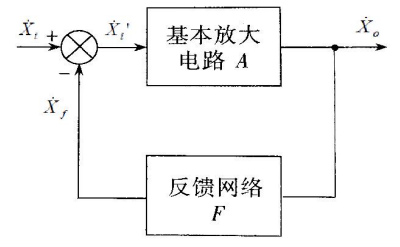
\includegraphics[width=.5\linewidth]{pic/1.png}
		\caption{反馈网络结构图
		}
	\end{figure}
\par 其中,$A $代表基本放大电路,$F $代表反馈网络,$X_{i}$为输入信号,$X_{f}$ 为反馈信号,$X_{o}$ 为输出信号,$X^{\prime}_{i}$为输入信号与反馈信号的差值。各变量之间的关系如下:$\dot{A}=\dfrac{\dot{X_{o}}}{\dot{X_{i}^{\prime}}},\dot{F}=\dfrac{\dot{X_{f}}}{\dot{X_{o}}},\dot{X_{i}^{\prime}}=\dot{X_{i}-\dot{X_{f}}}$
\par 由上式可得反馈电路闭环放大倍数$\dot{A_{f}}=\dfrac{\dot{A}}{1+\dot{A}\dot{F}}$
\par 本次实验实验电路如图二:
	\begin{figure}[H]
	\centering
	\hspace{2em}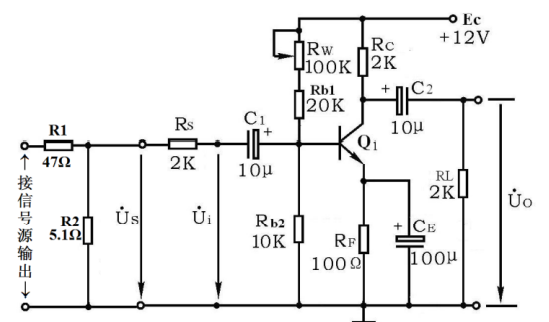
\includegraphics[width=.65\linewidth]{pic/2.png}
	\caption{实验电路图
	}
\end{figure}
\par 按照微变等效电路法计算可得:
\par 无反馈时放大倍数,输入阻抗和输出阻抗计算公式如下:$A=\dfrac{-\beta R_{L}^{\prime}}{r_{be}},R_{i}=r_{be}||(R_{b1}+R_{W})||R_{b2},R_{o}=R_{C}||r_{ce},R_{L}^{\prime}=R_{C}||R_{L}$
\par 有反馈时放大倍数,输入阻抗和输出阻抗计算公式如下:$A=\dfrac{-\beta R_{L}^{\prime}}{r_{be}+(1+\beta) R_{f}},R_{if}=[r_{be}+(1+\beta )R_{f}]||(R_{b1}+R_{W})||R_{b2},R_{of}=R_{C}||(r_{ce}+R_{e}^{\prime}+\frac{\beta r_{ce}}{r_{be}}R_{e}^{\prime}),R_{e}^{\prime}=R_{f}||r_{be}$
\par 其中$r_{ce}$为CE间内阻,一般很大,即有$r_{of}\approx R_{c}$。
\par 由上面公式可看出负反馈使电路的放大倍数下降,电流串联负反馈增大了输入电阻和输出电阻,从而改善了电路的性能。

	\section{实验内容}
	\noindent
	1.按照上图所示实验电路图插接面包板,2.调整电路的静态工作点,\\
	3.测量无反馈时的$A_{o},R_{i},R_{o}$,4.测量有反馈时的$A_{f},R_{if},R_{of}$
	\subsection{无反馈电路参数测量}
	\begin{figure}[H]
	\centering
	\hspace{2em}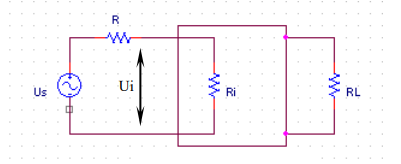
\includegraphics[width=.65\linewidth]{pic/3.png}
	\caption{无反馈等效电路图
	}
\end{figure}
\par 实验中记录$u_{i}=34.0mV,u_{o}=3.12V,u_{s}=70.0mV,u_{o\infty}=6.00V,R=1.963k\Omega,R_{l}=1.965k\Omega$
\par 因此计算可得:$A_{o}=\dfrac{u_{o}}{u_{i}}=91.8,R_{i}=\dfrac{Ru_{i}}{u_{s}-u_{i}}=1.851k\Omega,R_{o}=R_{l}(\dfrac{u_{o\infty}-u_{o}}{u_{o}})=1.813k\Omega$
\par 因此实验值与理论值(由实验原理部分计算可得)比较见下表:
\begin{table}[H]
	\centering
	\caption{无反馈系统参数实验值与理论值比较表}
	\begin{tabular}{|r|r|r|r|}
		\toprule[0.5mm]
		&$A_{o}$&$R_{i}/k\Omega$&$R_{o}/k\Omega$\\
		\midrule
		实验值&91.8&1.851&1.813\\
		\midrule
		理论值&88.9&1.827&1.875\\
		\bottomrule[0.5mm]
	\end{tabular}
\end{table}
	\subsection{有反馈电路参数测量}
		\begin{figure}[H]
		\centering
		\hspace{2em}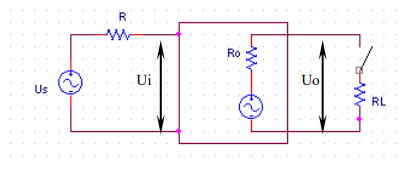
\includegraphics[width=.65\linewidth]{pic/4.png}
		\caption{有反馈等效电路图
		}
	\end{figure}
\par 实验中记录$u_{i}=47.2mV,u_{o}=448mV,u_{s}=61.2mV,u_{o\infty}=888mV,R=1.963k\Omega,R_{l}=1.965k\Omega$
\par 因此计算可得:$A_{F}=\dfrac{u_{o}}{u_{i}}=9.49,R_{iF}=\dfrac{Ru_{i}}{u_{s}-u_{i}}=6.623k\Omega,R_{oF}=R_{l}(\dfrac{u_{o\infty}-u_{o}}{u_{o}})=1.929k\Omega$
\par 因此实验值与理论值(由实验原理部分计算可得)比较见下表:
\begin{table}[H]
	\centering
	\caption{有反馈系统参数实验值与理论值比较表}
	\begin{tabular}{|r|r|r|r|}
		\toprule[0.5mm]
		&$A_{F}$&$R_{iF}/k\Omega$&$R_{oF}/\Omega$\\
		\midrule
		实验值&9.49&6.623&1.929\\
		\midrule
		理论值&9.95&6.543&1.987\\
		\bottomrule[0.5mm]
	\end{tabular}
\end{table}
\par \textbf{由以上数据可见负反馈使电路的放大倍数下降,电流串联负反馈增大了输入电阻和输出电阻,从而改善了电路的性能。}
	\section{思考题}
	\noindent
	\textbf{电流串联负反馈使输出阻抗增大,怎样解释本次实验中$r_{o}$与$r_{of}$几乎相等的现象?}
		\par 答:这是因为$r_{ce}$为管子CE间的内阻,一般阻值会很大,即满足关系$r_{ce}+R_{e}^{\prime}+\frac{\beta r_{ce}}{r_{be}}R_{e}^{\prime}$足够大,因此$r_{of}\approx R_{c}$,同理$r_{o}\approx R_{C}$,所以在本次实验中$r_{o}\approx r_{of}$。
	
	\begin{appendices}
		\section{原始数据整理}
		\begin{figure}[H]
	\centering
	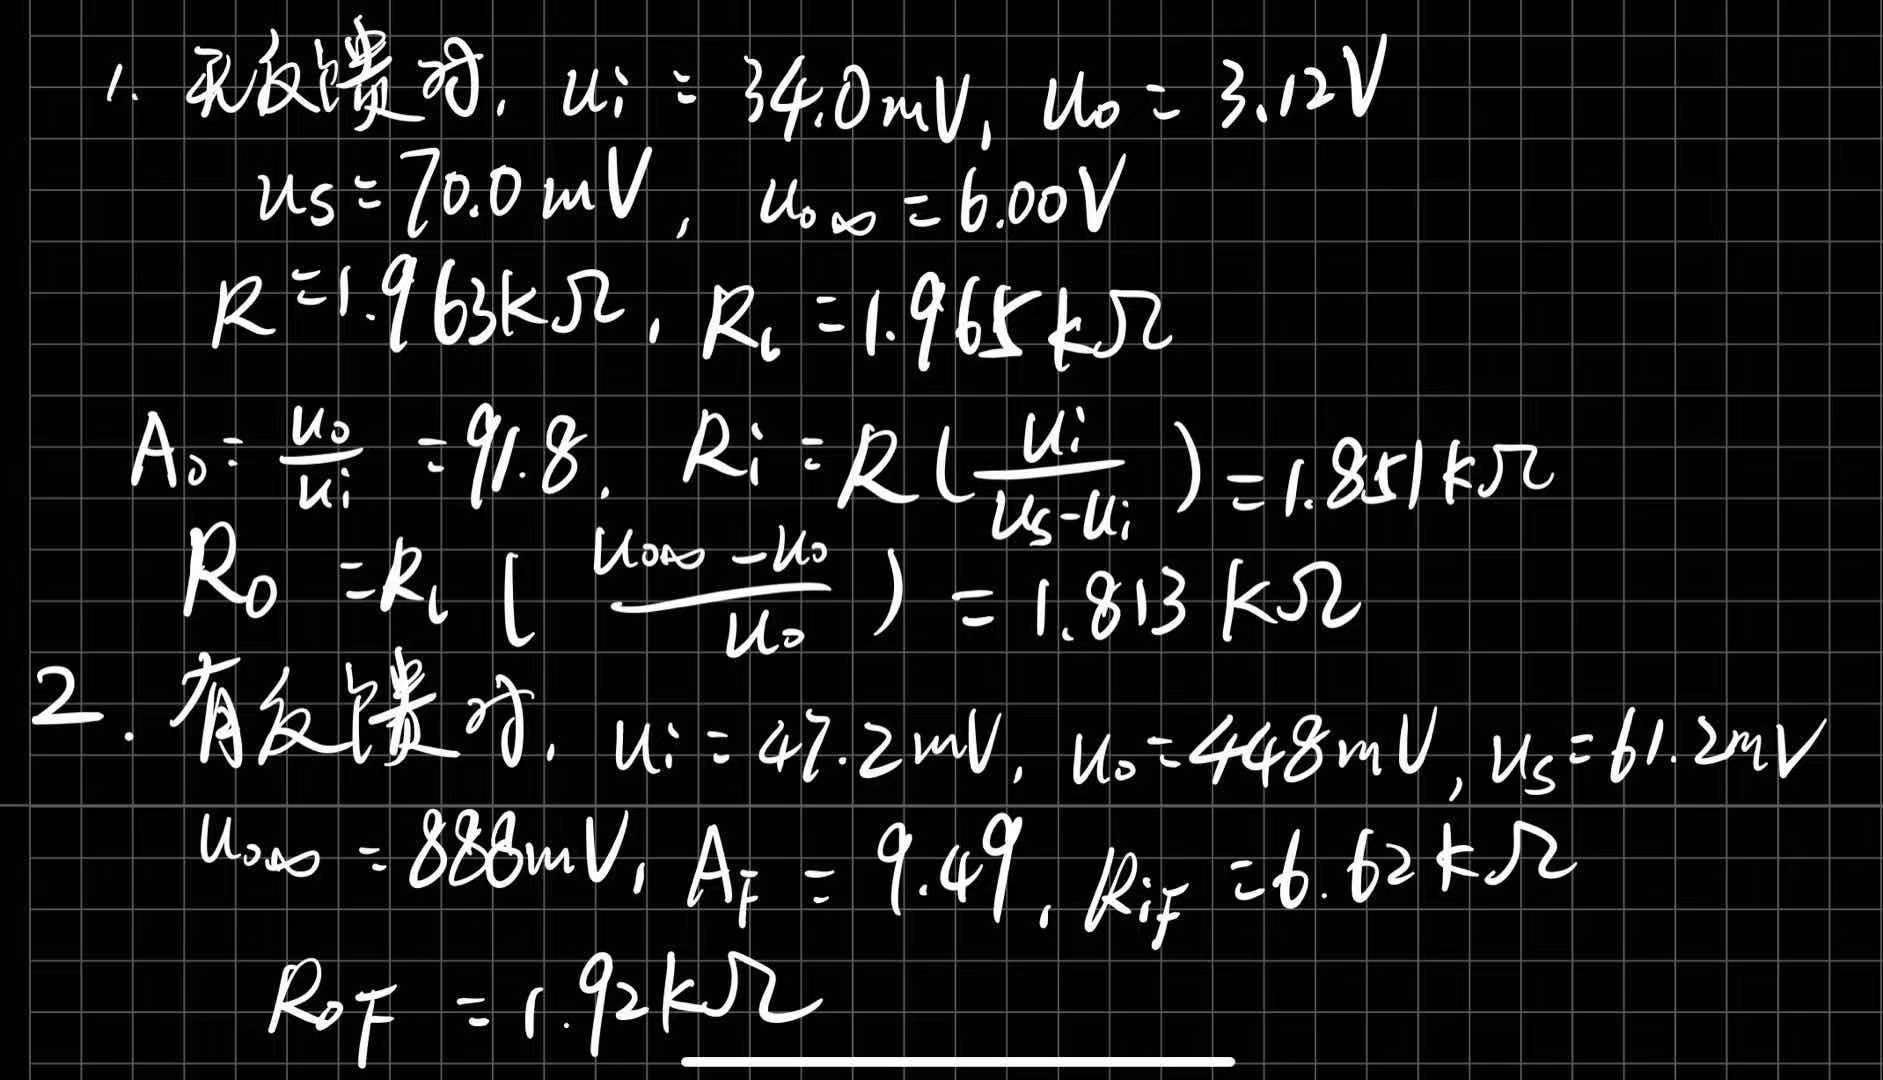
\includegraphics[width=.7\linewidth]{pic/1.jpg} 
	\caption{原始数据截图}
\end{figure}
	\end{appendices}
\end{document} 
